\documentclass{article}

% content/resources/templates/preamble.tex
\usepackage[margin=0.6in]{geometry}
\author{Milav Dabgar}
\usepackage{amsmath,amssymb,amsthm}
\usepackage{booktabs}
\usepackage{multirow}
\usepackage{xcolor}
\usepackage{tcolorbox}
\tcbuselibrary{breakable,skins}
\usepackage[colorlinks=true,linkcolor=blue]{hyperref}
\usepackage{titlesec}
\usepackage{enumitem}
\usepackage{tikz}
\usepackage{pgfplots}
\usepackage{circuitikz}
\usepackage[version=4]{mhchem}
\usepackage{longtable}
\usepackage{array}
\usepackage{float}
\usepackage{caption}
\usepackage{listings}

\lstset{
  basicstyle=\small\ttfamily,
  breaklines=true,
  breakatwhitespace=false,
  postbreak=\mbox{\textcolor{red}{$\hookrightarrow$}\space},
  float=false,
  numbers=left,
  numberstyle=\tiny\color{gray},
  numbersep=10pt,
  xleftmargin=2em,
  keywordstyle=\color{blue},
  commentstyle=\color{green!60!black},
  stringstyle=\color{purple},
  backgroundcolor=\color{gray!5},
  showstringspaces=false,
  tabsize=2,
  captionpos=b,
  keepspaces=true,
  columns=flexible
}

\pgfplotsset{compat=1.18}
\usetikzlibrary{shapes,arrows,positioning,calc,patterns,decorations.pathmorphing,decorations.markings,arrows.meta}

% Color scheme
\definecolor{headcolor}{RGB}{0,102,204}
\definecolor{keycolor}{RGB}{220,20,60}
\definecolor{solutioncolor}{RGB}{34,139,34}
\definecolor{mnemoniccolor}{RGB}{148,0,211}
\definecolor{codecolor}{RGB}{0,0,100}

% Spacing
\setlength{\parskip}{3pt}
\setlist[itemize]{nosep}
\setlist[enumerate]{nosep}

% Title formatting
\titleformat{\section}{\Large\bfseries\color{headcolor}}{\thesection}{1em}{}
\titleformat{\subsection}{\large\bfseries\color{headcolor}}{\thesubsection}{1em}{}

% Pandoc tightlist compatibility
\providecommand{\tightlist}{%
  \setlength{\itemsep}{0pt}\setlength{\parskip}{0pt}}

% Pandoc longtable compatibility
\newcounter{none}
\def\thenone{}


% content/resources/templates/english-boxes.tex

% Custom environments
\newtcolorbox{solutionbox}{
 breakable,
 enhanced,
 colback=solutioncolor!5!white,
 colframe=solutioncolor!75!black,
 fonttitle=\bfseries,
 title=Solution
}

\newtcolorbox{solutionboxnobreak}{
 colback=solutioncolor!5!white,
 colframe=solutioncolor!75!black,
 fonttitle=\bfseries,
 title=Solution
}

\newtcolorbox{keyformula}{
 breakable,
 enhanced,
 colback=keycolor!5!white,
 colframe=keycolor!75!black,
 fonttitle=\bfseries,
 title=Key Formula
}

\newtcolorbox{mnemonicboxenv}{
 breakable,
 enhanced,
 colback=mnemoniccolor!5!white,
 colframe=mnemoniccolor!75!black,
 fonttitle=\bfseries,
 title=Mnemonic
}

\newcommand{\mnemonicbox}[1]{%
  \begin{mnemonicboxenv}
    #1
  \end{mnemonicboxenv}
}


% Custom commands for GTU solutions
% This file defines semantic commands for consistent formatting

% Question command with automatic formatting
\newcommand{\question}[2]{%
  \section*{Question #1}%
  \textbf{#2}%
}

% OR question variant
\newcommand{\questionor}[2]{%
  \section*{Question #1 OR}%
  \textbf{#2}%
}

% Proper table environment with caption
\newenvironment{answertable}[1]{%
  \begin{table}[htbp]
  \centering
  \caption{#1}
}{%
  \end{table}
}

% Proper figure environment for diagrams
\newenvironment{answerdiagram}[1]{%
  \begin{figure}[htbp]
  \centering
  \caption{#1}
}{%
  \end{figure}
}

% Semantic markup for key terms
\newcommand{\keyword}[1]{\textbf{#1}}
\newcommand{\code}[1]{\texttt{#1}}
\newcommand{\classname}[1]{\texttt{#1}}
\newcommand{\methodname}[1]{\texttt{#1}}

% Proper quotation marks
\newcommand{\mnemonic}[1]{``#1''}


\title{Electronic Circuits \& Networks (4331101) - Summer 2025 Solution}
\date{May 9, 2025}

\begin{document}
\maketitle

\questionmarks{1(a)}{3}{Define following terms. (i) Active elements (ii) Bilateral elements (iii) Linear elements}

\begin{solutionbox}
\begin{center}
\begin{tabulary}{\linewidth}{|L|L|}
\hline
\textbf{Term} & \textbf{Definition} \\ \hline
\textbf{Active elements} & Electronic components that can supply energy or power to a circuit (like batteries, generators, op-amps) \\ \hline
\textbf{Bilateral elements} & Components that allow current flow equally in both directions with same characteristics (like resistors, capacitors, inductors) \\ \hline
\textbf{Linear elements} & Components whose current-voltage relationship follows a straight line and obeys the principle of superposition (like resistors following Ohm's law) \\ \hline
\end{tabulary}
\end{center}

\begin{mnemonicbox}
\mnemonic{ABL: Active powers Batteries, Bilateral flows Both ways, Linear stays Lawful}
\end{mnemonicbox}
\end{solutionbox}

\questionmarks{1(b)}{4}{Capacitors of 10$\mu$F, 20$\mu$F and 30$\mu$F are connected in series and supply of 200V DC is given. Find voltage across each capacitor.}

\begin{solutionbox}
For series-connected capacitors:
\begin{enumerate}
    \item Find equivalent capacitance: $1/C_{eq} = 1/C_1 + 1/C_2 + 1/C_3$
    \item Voltage division: $V_C = (C_{eq}/C_x) \times V$
\end{enumerate}

\textbf{Calculation:}
$1/C_{eq} = 1/10 + 1/20 + 1/30 = 0.1 + 0.05 + 0.033 = 0.183$
$C_{eq} = 5.46 \mu$F

\begin{center}
\begin{tabulary}{\linewidth}{|L|L|L|L|}
\hline
\textbf{Capacitor} & \textbf{Formula} & \textbf{Calculation} & \textbf{Voltage} \\ \hline
$C_1 = 10\mu$F & $V_1 = (C_{eq}/C_1) \times V$ & $(5.46/10) \times 200 = 109.2$V & 109.2V \\ \hline
$C_2 = 20\mu$F & $V_2 = (C_{eq}/C_2) \times V$ & $(5.46/20) \times 200 = 54.6$V & 54.6V \\ \hline
$C_3 = 30\mu$F & $V_3 = (C_{eq}/C_3) \times V$ & $(5.46/30) \times 200 = 36.4$V & 36.4V \\ \hline
\end{tabulary}
\end{center}

\begin{mnemonicbox}
\mnemonic{Smaller Capacitors get Larger Voltages}
\end{mnemonicbox}
\end{solutionbox}

\questionmarks{1(c)}{7}{Explain Node pair voltage method for graph theory.}

\begin{solutionbox}
Node pair voltage method is a systematic approach to analyze electrical networks.

\textbf{Procedure:}
\begin{enumerate}
    \item Select a reference node (ground)
    \item Identify the node voltages ($N-1$ unknowns for $N$ nodes)
    \item Apply KCL at each non-reference node
    \item Express branch currents in terms of node voltages
    \item Solve the equations for node voltages
\end{enumerate}

\begin{center}
\begin{tikzpicture}[node distance=2cm, auto, >=latex]
    \node[gtu block] (A) {Select reference node};
    \node[gtu block, right=of A] (B) {Identify node voltages};
    \node[gtu block, right=of B] (C) {Apply KCL at each node};
    \node[gtu block, below=of C] (D) {Express branch currents};
    \node[gtu block, left=of D] (E) {Solve equations};
    \node[gtu block, left=of E] (F) {Calculate currents};

    \draw[gtu arrow] (A) -- (B);
    \draw[gtu arrow] (B) -- (C);
    \draw[gtu arrow] (C) -- (D);
    \draw[gtu arrow] (D) -- (E);
    \draw[gtu arrow] (E) -- (F);
\end{tikzpicture}
\captionof{figure}{Node Pair Voltage Method Procedure}
\end{center}

\textbf{Key advantages:}
\begin{itemize}
    \item \textbf{Fewer equations}: Only ($n-1$) equations for $n$ nodes
    \item \textbf{Computational efficiency}: Reduces system complexity
    \item \textbf{Direct voltage solutions}: Provides node voltages directly
    \item \textbf{Systematic approach}: Works for any network topology
\end{itemize}

\begin{mnemonicbox}
\mnemonic{GARCS: Ground, Assign voltages, Relate with KCL, Calculate currents, Solve equations}
\end{mnemonicbox}
\end{solutionbox}

\questionmarks{1(c) OR}{7}{Explain voltage division method with necessary equations.}

\begin{solutionbox}
Voltage division is a method to calculate how voltage distributes across series components.

\textbf{Principle:}
In a series circuit, voltage divides proportionally to component resistances/impedances.

\textbf{Formula:}
For a resistor $R_1$ in a series circuit with total resistance $R_T$:
$V_1 = (R_1/R_T) \times V_S$

\begin{center}
\begin{circuitikz}[scale=1]
    \draw (0,0) to[V, l=$V_S$] (0,3) -- (2,3) to[R, l=$R_1$, v=$V_1$] (2,1.5);
    \draw (2,1.5) to[R, l=$R_2$] (2,0) -- (0,0);
\end{circuitikz}
\captionof{figure}{Voltage Divider Circuit}
\end{center}

\textbf{Mathematical explanation:}
\begin{itemize}
    \item For resistors: $V_1 = (R_1/R_T) \times V_S$
    \item For capacitors: $V_1 = (1/C_1)/(1/C_T) \times V_S = (C_T/C_1) \times V_S$
    \item For inductors: $V_1 = (L_1/L_T) \times V_S$
    \item For complex impedances: $V_1 = (Z_1/Z_T) \times V_S$
\end{itemize}

\textbf{Examples:}
\begin{enumerate}
    \item Voltage across a 1k$\Omega$ resistor in series with 4k$\Omega$ with 5V source = $(1/5) \times 5$V = 1V
    \item Voltage across a 10$\mu$F capacitor in series with 40$\mu$F with 10V source = $(1/10)/(1/8) \times 10$V = 8V
\end{enumerate}

\begin{mnemonicbox}
\mnemonic{The BIGGER the RESISTANCE, the BIGGER the VOLTAGE drop}
\end{mnemonicbox}
\end{solutionbox}

\questionmarks{2(a)}{3}{Write open circuit impedance parameters of Two port network.}

\begin{solutionbox}
\textbf{Open Circuit Impedance Parameters:}

\begin{center}
\begin{tabulary}{\linewidth}{|L|L|L|}
\hline
\textbf{Parameter} & \textbf{Equation} & \textbf{Physical Meaning} \\ \hline
\textbf{$Z_{11}$} & $Z_{11} = V_1/I_1$ (when $I_2=0$) & Input impedance with output open-circuited \\ \hline
\textbf{$Z_{12}$} & $Z_{12} = V_1/I_2$ (when $I_1=0$) & Transfer impedance from port 2 to port 1 \\ \hline
\textbf{$Z_{21}$} & $Z_{21} = V_2/I_1$ (when $I_2=0$) & Transfer impedance from port 1 to port 2 \\ \hline
\textbf{$Z_{22}$} & $Z_{22} = V_2/I_2$ (when $I_1=0$) & Output impedance with input open-circuited \\ \hline
\end{tabulary}
\end{center}

\begin{mnemonicbox}
\mnemonic{ZIPO: Z-parameters with Inputs and outputs, Ports Open where needed}
\end{mnemonicbox}
\end{solutionbox}

\questionmarks{2(b)}{4}{Derive conversion from T-type network to $\Pi$-type network.}

\begin{solutionbox}
\textbf{T to $\Pi$ Network Conversion:}

\begin{center}
\begin{tabular}{cc}
\begin{circuitikz}[scale=0.8]
    \node at (2,2.5) {\textbf{T-Network}};
    \draw (0,2) to[R, l=$Z_1$, o-] (2,2) to[R, l=$Z_2$, -o] (4,2);
    \draw (2,2) to[R, l=$Z_3$] (2,0) to[short] (0,0);
    \draw (2,0) to[short] (4,0);
\end{circuitikz} &
\begin{circuitikz}[scale=0.8]
    \node at (2,2.5) {\textbf{$\Pi$-Network}};
    \draw (0,2) to[R, l=$Y_1$ (series), o-o] (4,2);
    \draw (0,2) to[R, l=$Y_3$] (0,0);
    \draw (4,2) to[R, l=$Y_2$] (4,0);
    \draw (0,0) to[short] (4,0);
\end{circuitikz}
\end{tabular}
\captionof{figure}{T and $\Pi$ Network Conversion}
\end{center}

\textbf{Conversion Equations:}

\begin{center}
\begin{tabulary}{\linewidth}{|L|L|L|}
\hline
\textbf{$\Pi$-Parameter} & \textbf{Formula} & \textbf{Based on T-Parameters} \\ \hline
$Y_1 = 1/Z_{\pi1}$ & $Y_1 = Z_2/(Z_1Z_2+Z_2Z_3+Z_3Z_1)$ & Reciprocal of $Z_1$ equivalent \\ \hline
$Y_2 = 1/Z_{\pi2}$ & $Y_2 = Z_1/(Z_1Z_2+Z_2Z_3+Z_3Z_1)$ & Reciprocal of $Z_2$ equivalent \\ \hline
$Y_3 = 1/Z_{\pi3}$ & $Y_3 = Z_3/(Z_1Z_2+Z_2Z_3+Z_3Z_1)$ & Reciprocal of $Z_3$ equivalent \\ \hline
\end{tabulary}
\end{center}

\textbf{Derivation Steps:}
\begin{enumerate}
    \item Define determinant $\Delta = Z_1Z_2+Z_2Z_3+Z_3Z_1$
    \item Use network theory to derive $Y_1 = Z_2/\Delta$
    \item Similarly, $Y_2 = Z_1/\Delta$ and $Y_3 = Z_3/\Delta$
\end{enumerate}

\begin{mnemonicbox}
\mnemonic{Delta Divides: Y1 gets Z2, Y2 gets Z1, Y3 gets Z3}
\end{mnemonicbox}
\end{solutionbox}

\questionmarks{2(c)}{7}{Three resistances of 1, 1 and 1 ohms are connected in Delta. Find equivalent resistances in star connection.}

\begin{solutionbox}
\textbf{Delta to Star Conversion:}

\begin{center}
\begin{tabular}{cc}
\begin{circuitikz}[scale=0.8]
    \node at (1.5,2) {\textbf{Delta}};
    \draw (0,0) to[R, l=$R_3$] (1.5,2.6) to[R, l=$R_1$] (3,0) to[R, l=$R_2$] (0,0);
\end{circuitikz} &
\begin{circuitikz}[scale=0.8]
    \node at (1.5,2) {\textbf{Star}};
    \draw (0,0) node[anchor=east]{B} to[R, l=$r_b$] (1.5,1) to[R, l=$r_a$] (1.5,2.6) node[anchor=south]{A};
    \draw (1.5,1) to[R, l=$r_c$] (3,0) node[anchor=west]{C};
\end{circuitikz}
\end{tabular}
\captionof{figure}{Delta to Star Conversion}
\end{center}

\textbf{Conversion Formulas:}
\begin{itemize}
    \item $r_a = (R_1 \times R_3)/(R_1+R_2+R_3)$
    \item $r_b = (R_1 \times R_2)/(R_1+R_2+R_3)$
    \item $r_c = (R_2 \times R_3)/(R_1+R_2+R_3)$
\end{itemize}

\textbf{Calculation:}
Given: $R_1 = R_2 = R_3 = 1\Omega$
Sum of resistances: $R_1+R_2+R_3 = 3\Omega$

\begin{center}
\begin{tabulary}{\linewidth}{|L|L|L|L|}
\hline
\textbf{Star Resistor} & \textbf{Formula} & \textbf{Calculation} & \textbf{Result} \\ \hline
$r_a$ & $(R_1 \times R_3)/\Sigma R$ & $(1 \times 1)/3$ & $0.333\Omega$ \\ \hline
$r_b$ & $(R_1 \times R_2)/\Sigma R$ & $(1 \times 1)/3$ & $0.333\Omega$ \\ \hline
$r_c$ & $(R_2 \times R_3)/\Sigma R$ & $(1 \times 1)/3$ & $0.333\Omega$ \\ \hline
\end{tabulary}
\end{center}

\begin{mnemonicbox}
\mnemonic{Product Over Sum: Each star arm gets the product of adjacent delta sides divided by the sum of all}
\end{mnemonicbox}
\end{solutionbox}

\questionmarks{2(a) OR}{3}{Define. (i) Transfer Impedance (ii) Image Impedance (iii) Driving point Impedance}

\begin{solutionbox}
\begin{center}
\begin{tabulary}{\linewidth}{|L|L|}
\hline
\textbf{Term} & \textbf{Definition} \\ \hline
\textbf{Transfer Impedance} & Ratio of output voltage at one port to input current at another port when all other ports are open-circuited ($Z_{21} = V_2/I_1$ when $I_2=0$) \\ \hline
\textbf{Image Impedance} & Input impedance at port when the output port is terminated with its own image impedance, creating infinite chain with same impedance at all points \\ \hline
\textbf{Driving point Impedance} & Input impedance seen when looking into a specified port or terminal pair ($Z_{11} = V_1/I_1$ for port 1) \\ \hline
\end{tabulary}
\end{center}

\begin{mnemonicbox}
\mnemonic{TID: Transfer relates ports, Image creates reflections, Driving point looks inward}
\end{mnemonicbox}
\end{solutionbox}

\questionmarks{2(b) OR}{4}{Get the equation for characteristics impedance Z for a standard 'T' network.}

\begin{solutionbox}
\textbf{Characteristic Impedance of 'T' network:}

\begin{center}
\begin{circuitikz}[scale=1]
    \draw (0,2) to[R, l=$Z_1/2$, o-] (2,2) to[R, l=$Z_1/2$, -o] (4,2);
    \draw (2,2) to[R, l=$Z_2$] (2,0) node[ground]{};
    \draw (0,0) to[short, o-o] (4,0);
\end{circuitikz}
\captionof{figure}{Symmetrical T-Network}
\end{center}

\textbf{Derivation:}
For a symmetrical T-network with series impedance $Z_1$ (split as $Z_1/2$ on each side) and shunt impedance $Z_2$:
$Z_0 = \sqrt{Z_1Z_2 + Z_1^2/4}$

\textbf{Steps:}
\begin{enumerate}
    \item ABCD parameters for T-network:
    \begin{itemize}
        \item $A = 1 + Z_1/2Z_2$
        \item $B = Z_1 + Z_1^2/4Z_2$
        \item $C = 1/Z_2$
        \item $D = 1 + Z_1/2Z_2$
    \end{itemize}
    \item From transmission line theory, $Z_0 = \sqrt{B/C}$
    \item Substituting: $Z_0 = \sqrt{(Z_1 + Z_1^2/4Z_2)/(1/Z_2)}$
    \item Simplifying: $Z_0 = \sqrt{Z_1Z_2 + Z_1^2/4}$
\end{enumerate}

\begin{mnemonicbox}
\mnemonic{Square root of Z-products plus quarter-square}
\end{mnemonicbox}
\end{solutionbox}

\questionmarks{2(c) OR}{7}{Three resistances of 6, 15 and 10 ohms are connected in star. Find equivalent resistances in delta connection.}

\begin{solutionbox}
\textbf{Star to Delta Conversion:}

\begin{center}
\begin{tabular}{cc}
\begin{circuitikz}[scale=0.8]
    \node at (1.5,2) {\textbf{Star}};
    \draw (0,0) node[anchor=east]{B} to[R, l=$r_b$, *-] (1.5,1) to[R, l=$r_a$, -*] (1.5,2.6) node[anchor=south]{A};
    \draw (1.5,1) to[R, l=$r_c$, -*] (3,0) node[anchor=west]{C};
\end{circuitikz} &
\begin{circuitikz}[scale=0.8]
    \node at (1.5,2) {\textbf{Delta}};
    \draw (0,0) to[R, l=$R_3$] (1.5,2.6) to[R, l=$R_1$] (3,0) to[R, l=$R_2$] (0,0);
\end{circuitikz}
\end{tabular}
\captionof{figure}{Star to Delta Conversion}
\end{center}

\textbf{Conversion Formulas:}
\begin{itemize}
    \item $R_1 = (r_a r_b + r_b r_c + r_c r_a)/r_a$
    \item $R_2 = (r_a r_b + r_b r_c + r_c r_a)/r_b$
    \item $R_3 = (r_a r_b + r_b r_c + r_c r_a)/r_c$
\end{itemize}

\textbf{Calculation:}
Given: $r_a = 6\Omega, r_b = 15\Omega, r_c = 10\Omega$
Sum of products = $(6 \times 15) + (15 \times 10) + (10 \times 6) = 90 + 150 + 60 = 300$

\begin{center}
\begin{tabulary}{\linewidth}{|L|L|L|L|}
\hline
\textbf{Delta Resistor} & \textbf{Formula} & \textbf{Calculation} & \textbf{Result} \\ \hline
$R_1$ & Sum of Products/$r_a$ & $300/6$ & $50\Omega$ \\ \hline
$R_2$ & Sum of Products/$r_b$ & $300/15$ & $20\Omega$ \\ \hline
$R_3$ & Sum of Products/$r_c$ & $300/10$ & $30\Omega$ \\ \hline
\end{tabulary}
\end{center}

\begin{mnemonicbox}
\mnemonic{Sum of Products Over Each: Delta side gets all products divided by opposite star arm}
\end{mnemonicbox}
\end{solutionbox}

\questionmarks{3(a)}{3}{Analyze the circuit (R1, R2 and R3 Connected in series with dc supply) to calculate loop current using KVL.}

\begin{solutionbox}
\textbf{KVL for Series Circuit:}

\begin{center}
\begin{circuitikz}[scale=1]
    \draw (0,0) to[V, l=$V_S$] (0,3) to[R, l=$R_1$] (3,3) to[R, l=$R_2$] (6,3) to[R, l=$R_3$] (6,0) -- (0,0);
    \draw[->, thick, blue] (2, 1.5) arc (120:-120:0.5) node[right] {$I$};
\end{circuitikz}
\captionof{figure}{Series Circuit for KVL}
\end{center}

\textbf{KVL Equation:} $V_S - IR_1 - IR_2 - IR_3 = 0$

\textbf{Loop Current:} $I = V_S/(R_1 + R_2 + R_3)$

\textbf{Steps:}
\begin{enumerate}
    \item Identify all elements in the loop: $V_S, R_1, R_2, R_3$
    \item Apply KVL: Sum of voltage rises = Sum of voltage drops
    \item Solve for $I$: $I = V_S/R_{eq}$ where $R_{eq} = R_1 + R_2 + R_3$
\end{enumerate}

\begin{mnemonicbox}
\mnemonic{KVL: Kirchhoff's Voltage Loop requires total resistance}
\end{mnemonicbox}
\end{solutionbox}

\questionmarks{3(b)}{4}{State Norton's theorem}

\begin{solutionbox}
\textbf{Norton's Theorem:}
Any linear electrical network consisting of voltage sources, current sources, and resistances can be replaced by an equivalent circuit consisting of a current source $I_N$ in parallel with a resistance $R_N$.

\begin{center}
\begin{circuitikz}[scale=0.9]
    \node[gtu block] (A) {Linear Network};
    \draw (A.east) -- ++(1,0) node[right] {Load};
    
    \draw[->, very thick] (3,0) -- (4,0) node[midway, above] {Equivalent};
    
    \draw (5,0) to[I, l=$I_N$] (5,2) -- (7,2);
    \draw (5,0) -- (7,0);
    \draw (7,2) to[R, l=$R_N$] (7,0);
    \draw (7,2) -- (8,2) node[right, o-o] {Load};
    \draw (7,0) -- (8,0);
\end{circuitikz}
\captionof{figure}{Norton's Equivalent Circuit}
\end{center}

\textbf{How to find Norton equivalent:}
\begin{enumerate}
    \item \textbf{Norton Current ($I_N$)}: Short-circuit current flowing through the load terminals
    \item \textbf{Norton Resistance ($R_N$)}: Input resistance seen at the terminals with all sources replaced by their internal resistances
\end{enumerate}

\begin{mnemonicbox}
\mnemonic{SCIP: Short-Circuit current In Parallel with equivalent resistance}
\end{mnemonicbox}
\end{solutionbox}

\questionmarks{3(c)}{7}{Explain the steps to calculate the current in any branch of the ckt using superposition theorem}

\begin{solutionbox}
\textbf{Superposition Theorem Application:}

\textbf{Principle:}
In a linear circuit with multiple sources, the response in any element equals the sum of responses caused by each source acting alone.

\textbf{Steps:}
\begin{enumerate}
    \item Consider only one source at a time
    \item Replace other voltage sources with short circuits
    \item Replace other current sources with open circuits
    \item Calculate partial current for each source
    \item Add all partial currents (algebraically) for final current
\end{enumerate}

\begin{center}
\begin{tikzpicture}[node distance=2cm, auto, >=latex]
    \node[gtu block] (A) {Select one source};
    \node[gtu block, right=of A] (B) {Replace other sources};
    \node[gtu block, right=of B] (C) {Calculate partial current};
    \node[gtu block, below=of C] (D) {Repeat for all sources};
    \node[gtu block, left=of D] (E) {Sum partial currents};
    
    \draw[gtu arrow] (A) -- (B);
    \draw[gtu arrow] (B) -- (C);
    \draw[gtu arrow] (C) -- (D);
    \draw[gtu arrow] (D) -- (E);
\end{tikzpicture}
\captionof{figure}{Superposition Process}
\end{center}

\textbf{Mathematical Expression:}
$I = I_1 + I_2 + I_3 + ... + I_n$
where $I_1, I_2$, etc. are partial currents due to individual sources

\textbf{Example calculation:}
For a branch with current contributions:
$I_1 = 2A$ (from source 1)
$I_2 = -1A$ (from source 2)
$I_3 = 0.5A$ (from source 3)
Total current = $2A + (-1A) + 0.5A = 1.5A$

\begin{mnemonicbox}
\mnemonic{OSACI: One Source Active, Calculate and Integrate}
\end{mnemonicbox}
\end{solutionbox}

\questionmarks{3(a) OR}{3}{Analyze the circuit (R1, R2 and R3 Connected in parallel with dc supply) to calculate node voltage using KCL.}

\begin{solutionbox}
\textbf{KCL for Parallel Circuit:}

\begin{center}
\begin{circuitikz}[scale=1]
    \draw (0,0) to[V, l=$V_S$] (0,3) -- (6,3);
    \draw (0,0) -- (6,0);
    \draw (2,3) to[R, l=$R_1$, i=$I_1$] (2,0);
    \draw (4,3) to[R, l=$R_2$, i=$I_2$] (4,0);
    \draw (6,3) to[R, l=$R_3$, i=$I_3$] (6,0);
    \node at (6,3) [label=above:Node V]{};
\end{circuitikz}
\captionof{figure}{Parallel Circuit for KCL}
\end{center}

\textbf{KCL Equation:} $I_1 + I_2 + I_3 = I_{total}$ (if current source) or simply sum of currents from node is zero.
Here connected to DC supply $V_S$:
Since parallel, Voltage across each $R$ is $V_S$.
Node Voltage $V = V_S$.

\textbf{Steps:}
\begin{enumerate}
    \item Identify node voltage $V$
    \item Express branch currents: $I_1 = V/R_1, I_2 = V/R_2, I_3 = V/R_3$
    \item Apply KCL if there was a current source. For Voltage source, $V$ is known.
    \item If $V_S$ connected via series resistor, then $V/R_1 + V/R_2 + V/R_3 = (V_S-V)/R_{series}$.
\end{enumerate}

\begin{mnemonicbox}
\mnemonic{KCL: Kirchhoff's Current Law means parallel voltage equals source}
\end{mnemonicbox}
\end{solutionbox}

\questionmarks{3(b) OR}{4}{State Maximum power transfer theorem.}

\begin{solutionbox}
\textbf{Maximum Power Transfer Theorem:}
For a source with internal resistance, maximum power is transferred to the load when the load resistance equals the source's internal resistance.

\begin{center}
\begin{circuitikz}[scale=1]
    \draw (0,0) to[V, l=$V_{th}$] (0,2) to[R, l=$R_{th}$] (3,2) to[R, l=$R_L$] (3,0) -- (0,0);
\end{circuitikz}
\captionof{figure}{Maximum Power Transfer Circuit}
\end{center}

\textbf{Mathematical expression:}
\begin{itemize}
    \item Maximum power transfer occurs when $R_L = R_{source}$ (or $R_{th}$)
    \item Maximum power: $P_{max} = V_{th}^2/(4 \times R_{th})$
\end{itemize}

\textbf{Key points:}
\begin{itemize}
    \item \textbf{Efficiency}: Only 50\% at maximum power transfer
    \item \textbf{AC Circuits}: Load impedance must be complex conjugate of source impedance ($Z_L = Z_S^*$)
    \item \textbf{Applications}: Signal transmission, audio systems, RF circuits
\end{itemize}

\begin{mnemonicbox}
\mnemonic{MEET: Maximum Efficiency Equals when Thevenin-matched}
\end{mnemonicbox}
\end{solutionbox}

\questionmarks{3(c) OR}{7}{Explain the steps to calculate Vth, Rth and load current in the ckt using Thevenin's theorem}

\begin{solutionbox}
\textbf{Thevenin's Theorem Application:}

\textbf{Principle:}
Any linear electrical network with voltage and current sources can be replaced by an equivalent circuit with a single voltage source $V_{th}$ and a series resistance $R_{th}$.

\textbf{Steps:}
\begin{enumerate}
    \item Remove the load resistance from the circuit
    \item Calculate open-circuit voltage ($V_{th}$) across the load terminals
    \item Replace all sources with their internal resistances (voltage sources as short circuits, current sources as open circuits)
    \item Calculate equivalent resistance ($R_{th}$) seen from the load terminals
    \item Draw the Thevenin equivalent circuit with $V_{th}$ and $R_{th}$
    \item Reconnect the load and calculate load current: $I_L = V_{th}/(R_{th} + R_L)$
\end{enumerate}

\begin{center}
\begin{tikzpicture}[node distance=2cm, auto, >=latex]
    \node[gtu block] (A) {Remove load};
    \node[gtu block, right=of A] (B) {Find $V_{th}$};
    \node[gtu block, right=of B] (C) {Kill sources};
    \node[gtu block, below=of C] (D) {Calculate $R_{th}$};
    \node[gtu block, left=of D] (E) {Draw Equivalent};
    \node[gtu block, left=of E] (F) {Calc $I_L$};
    
    \draw[gtu arrow] (A) -- (B);
    \draw[gtu arrow] (B) -- (C);
    \draw[gtu arrow] (C) -- (D);
    \draw[gtu arrow] (D) -- (E);
    \draw[gtu arrow] (E) -- (F);
\end{tikzpicture}
\captionof{figure}{Thevenin's Procedure}
\end{center}

\textbf{Example calculation:}
\begin{itemize}
    \item If $V_{th} = 12V$
    \item $R_{th} = 3\Omega$
    \item $R_L = 6\Omega$
    \item Then $I_L = 12V/(3\Omega + 6\Omega) = 12V/9\Omega = 1.33A$
\end{itemize}

\begin{mnemonicbox}
\mnemonic{VORTE: Voltage Open, Resistance with sources Transformed, Equivalent circuit}
\end{mnemonicbox}
\end{solutionbox}

\questionmarks{3(a)}{3}{Analyze the circuit (R1, R2 and R3 Connected in series with dc supply) to calculate loop current using KVL.}

\begin{solutionbox}
\textbf{KVL for Series Circuit:}

\begin{center}
\begin{circuitikz}[scale=1]
    \draw (0,0) to[V, l=$V_S$] (0,3) to[R, l=$R_1$] (3,3) to[R, l=$R_2$] (6,3) to[R, l=$R_3$] (6,0) -- (0,0);
    \draw[->, thick, blue] (2, 1.5) arc (120:-120:0.5) node[right] {$I$};
\end{circuitikz}
\captionof{figure}{Series Circuit for KVL}
\end{center}

\textbf{KVL Equation:} $V_S - IR_1 - IR_2 - IR_3 = 0$

\textbf{Loop Current:} $I = V_S/(R_1 + R_2 + R_3)$

\textbf{Steps:}
\begin{enumerate}
    \item Identify all elements in the loop: $V_S, R_1, R_2, R_3$
    \item Apply KVL: Sum of voltage rises = Sum of voltage drops
    \item Solve for $I$: $I = V_S/R_{eq}$ where $R_{eq} = R_1 + R_2 + R_3$
\end{enumerate}

\begin{mnemonicbox}
\mnemonic{KVL: Kirchhoff's Voltage Loop requires total resistance}
\end{mnemonicbox}
\end{solutionbox}

\questionmarks{3(b)}{4}{State Norton's theorem}

\begin{solutionbox}
\textbf{Norton's Theorem:}
Any linear electrical network consisting of voltage sources, current sources, and resistances can be replaced by an equivalent circuit consisting of a current source $I_N$ in parallel with a resistance $R_N$.

\begin{center}
\begin{circuitikz}[scale=0.9]
    \node[gtu block] (A) {Linear Network};
    \draw (A.east) -- ++(1,0) node[right] {Load};
    
    \draw[->, very thick] (3,0) -- (4,0) node[midway, above] {Equivalent};
    
    \draw (5,0) to[I, l=$I_N$] (5,2) -- (7,2);
    \draw (5,0) -- (7,0);
    \draw (7,2) to[R, l=$R_N$] (7,0);
    \draw (7,2) -- (8,2) node[right, o-o] {Load};
    \draw (7,0) -- (8,0);
\end{circuitikz}
\captionof{figure}{Norton's Equivalent Circuit}
\end{center}

\textbf{How to find Norton equivalent:}
\begin{enumerate}
    \item \textbf{Norton Current ($I_N$)}: Short-circuit current flowing through the load terminals
    \item \textbf{Norton Resistance ($R_N$)}: Input resistance seen at the terminals with all sources replaced by their internal resistances
\end{enumerate}

\begin{mnemonicbox}
\mnemonic{SCIP: Short-Circuit current In Parallel with equivalent resistance}
\end{mnemonicbox}
\end{solutionbox}

\questionmarks{3(c)}{7}{Explain the steps to calculate the current in any branch of the ckt using superposition theorem}

\begin{solutionbox}
\textbf{Superposition Theorem Application:}

\textbf{Principle:}
In a linear circuit with multiple sources, the response in any element equals the sum of responses caused by each source acting alone.

\textbf{Steps:}
\begin{enumerate}
    \item Consider only one source at a time
    \item Replace other voltage sources with short circuits
    \item Replace other current sources with open circuits
    \item Calculate partial current for each source
    \item Add all partial currents (algebraically) for final current
\end{enumerate}

\begin{center}
\begin{tikzpicture}[node distance=2cm, auto, >=latex]
    \node[gtu block] (A) {Select one source};
    \node[gtu block, right=of A] (B) {Replace other sources};
    \node[gtu block, right=of B] (C) {Calculate partial current};
    \node[gtu block, below=of C] (D) {Repeat for all sources};
    \node[gtu block, left=of D] (E) {Sum partial currents};
    
    \draw[gtu arrow] (A) -- (B);
    \draw[gtu arrow] (B) -- (C);
    \draw[gtu arrow] (C) -- (D);
    \draw[gtu arrow] (D) -- (E);
\end{tikzpicture}
\captionof{figure}{Superposition Process}
\end{center}

\textbf{Mathematical Expression:}
$I = I_1 + I_2 + I_3 + ... + I_n$
where $I_1, I_2$, etc. are partial currents due to individual sources

\textbf{Example calculation:}
For a branch with current contributions:
$I_1 = 2A$ (from source 1)
$I_2 = -1A$ (from source 2)
$I_3 = 0.5A$ (from source 3)
Total current = $2A + (-1A) + 0.5A = 1.5A$

\begin{mnemonicbox}
\mnemonic{OSACI: One Source Active, Calculate and Integrate}
\end{mnemonicbox}
\end{solutionbox}

\questionmarks{3(a) OR}{3}{Analyze the circuit (R1, R2 and R3 Connected in parallel with dc supply) to calculate node voltage using KCL.}

\begin{solutionbox}
\textbf{KCL for Parallel Circuit:}

\begin{center}
\begin{circuitikz}[scale=1]
    \draw (0,0) to[V, l=$V_S$] (0,3) -- (6,3);
    \draw (0,0) -- (6,0);
    \draw (2,3) to[R, l=$R_1$, i=$I_1$] (2,0);
    \draw (4,3) to[R, l=$R_2$, i=$I_2$] (4,0);
    \draw (6,3) to[R, l=$R_3$, i=$I_3$] (6,0);
    \node at (6,3) [label=above:Node V]{};
\end{circuitikz}
\captionof{figure}{Parallel Circuit for KCL}
\end{center}

\textbf{KCL Equation:} $I_1 + I_2 + I_3 = I_{total}$ (if current source) or simply sum of currents from node is zero.
Here connected to DC supply $V_S$:
Since parallel, Voltage across each $R$ is $V_S$.
Node Voltage $V = V_S$.

\textbf{Steps:}
\begin{enumerate}
    \item Identify node voltage $V$
    \item Express branch currents: $I_1 = V/R_1, I_2 = V/R_2, I_3 = V/R_3$
    \item Apply KCL if there was a current source. For Voltage source, $V$ is known.
    \item If $V_S$ connected via series resistor, then $V/R_1 + V/R_2 + V/R_3 = (V_S-V)/R_{series}$.
\end{enumerate}

\begin{mnemonicbox}
\mnemonic{KCL: Kirchhoff's Current Law means parallel voltage equals source}
\end{mnemonicbox}
\end{solutionbox}

\questionmarks{3(b) OR}{4}{State Maximum power transfer theorem.}

\begin{solutionbox}
\textbf{Maximum Power Transfer Theorem:}
For a source with internal resistance, maximum power is transferred to the load when the load resistance equals the source's internal resistance.

\begin{center}
\begin{circuitikz}[scale=1]
    \draw (0,0) to[V, l=$V_{th}$] (0,2) to[R, l=$R_{th}$] (3,2) to[R, l=$R_L$] (3,0) -- (0,0);
\end{circuitikz}
\captionof{figure}{Maximum Power Transfer Circuit}
\end{center}

\textbf{Mathematical expression:}
\begin{itemize}
    \item Maximum power transfer occurs when $R_L = R_{source}$ (or $R_{th}$)
    \item Maximum power: $P_{max} = V_{th}^2/(4 \times R_{th})$
\end{itemize}

\textbf{Key points:}
\begin{itemize}
    \item \textbf{Efficiency}: Only 50\% at maximum power transfer
    \item \textbf{AC Circuits}: Load impedance must be complex conjugate of source impedance ($Z_L = Z_S^*$)
    \item \textbf{Applications}: Signal transmission, audio systems, RF circuits
\end{itemize}

\begin{mnemonicbox}
\mnemonic{MEET: Maximum Efficiency Equals when Thevenin-matched}
\end{mnemonicbox}
\end{solutionbox}

\questionmarks{3(c) OR}{7}{Explain the steps to calculate Vth, Rth and load current in the ckt using Thevenin's theorem}

\begin{solutionbox}
\textbf{Thevenin's Theorem Application:}

\textbf{Principle:}
Any linear electrical network with voltage and current sources can be replaced by an equivalent circuit with a single voltage source $V_{th}$ and a series resistance $R_{th}$.

\textbf{Steps:}
\begin{enumerate}
    \item Remove the load resistance from the circuit
    \item Calculate open-circuit voltage ($V_{th}$) across the load terminals
    \item Replace all sources with their internal resistances (voltage sources as short circuits, current sources as open circuits)
    \item Calculate equivalent resistance ($R_{th}$) seen from the load terminals
    \item Draw the Thevenin equivalent circuit with $V_{th}$ and $R_{th}$
    \item Reconnect the load and calculate load current: $I_L = V_{th}/(R_{th} + R_L)$
\end{enumerate}

\begin{center}
\begin{tikzpicture}[node distance=2cm, auto, >=latex]
    \node[gtu block] (A) {Remove load};
    \node[gtu block, right=of A] (B) {Find $V_{th}$};
    \node[gtu block, right=of B] (C) {Kill sources};
    \node[gtu block, below=of C] (D) {Calculate $R_{th}$};
    \node[gtu block, left=of D] (E) {Draw Equivalent};
    \node[gtu block, left=of E] (F) {Calc $I_L$};
    
    \draw[gtu arrow] (A) -- (B);
    \draw[gtu arrow] (B) -- (C);
    \draw[gtu arrow] (C) -- (D);
    \draw[gtu arrow] (D) -- (E);
    \draw[gtu arrow] (E) -- (F);
\end{tikzpicture}
\captionof{figure}{Thevenin's Procedure}
\end{center}

\textbf{Example calculation:}
\begin{itemize}
    \item If $V_{th} = 12V$
    \item $R_{th} = 3\Omega$
    \item $R_L = 6\Omega$
    \item Then $I_L = 12V/(3\Omega + 6\Omega) = 12V/9\Omega = 1.33A$
\end{itemize}

\begin{mnemonicbox}
\mnemonic{VORTE: Voltage Open, Resistance with sources Transformed, Equivalent circuit}
\end{mnemonicbox}
\end{solutionbox}

\questionmarks{4(a)}{3}{Draw a coupled circuit. Mark L1, L2 and M.}

\begin{solutionbox}
\textbf{Coupled Circuit Diagram:}

\begin{center}
\begin{circuitikz}[scale=1]
    \draw (0,0) to[L, l=$L_1$, name=L1] (0,2);
    \draw (2,2) to[L, l=$L_2$, name=L2] (2,0);
    \draw (0,0) -- (2,0);
    \draw (0,2) -- (-1,2) node[left] {Input};
    \draw (2,2) -- (3,2) node[right] {Output};
    
    % Mutual inductance symbol
    \draw [densely dashed, <->] (0.4,1) -- (1.6,1) node[midway, above] {$M$};
    
    % Dot convention
    \node [circle, fill, inner sep=1pt] at (-0.2, 1.8) {};
    \node [circle, fill, inner sep=1pt] at (1.8, 1.8) {};
\end{circuitikz}
\captionof{figure}{Magnetically Coupled Circuit}
\end{center}

\textbf{Components:}
\begin{itemize}
    \item $L_1$: Self-inductance of coil 1
    \item $L_2$: Self-inductance of coil 2
    \item $M$: Mutual inductance between coils
    \item Dots indicate polarity of induced voltage
\end{itemize}

\begin{mnemonicbox}
\mnemonic{M-Link: Mutual inductance links two coils together}
\end{mnemonicbox}
\end{solutionbox}

\questionmarks{4(b)}{4}{Define coefficient of coupling. State the relation K, M, L1, L2.}

\begin{solutionbox}
\textbf{Coefficient of Coupling ($K$):}
The fraction of magnetic flux produced by one coil that links with the other coil. It represents the extent of magnetic coupling between two coils.

\textbf{Relation:}
$M = K\sqrt{L_1 L_2}$
or
$K = M/\sqrt{L_1 L_2}$

\textbf{Key properties:}
\begin{itemize}
    \item Range: $0 \le K \le 1$
    \item $K=1$: Perfectly coupled (tight coupling)
    \item $K=0$: No coupling (magnetically isolated)
    \item $K<0.5$: Loosely coupled
\end{itemize}

\begin{mnemonicbox}
\mnemonic{K defines the Link: Ratio of Mutual to Geometric Mean of Selfs}
\end{mnemonicbox}
\end{solutionbox}

\questionmarks{4(c)}{7}{Derive equation for resonant frequency of series resonance circuit. A series RLC circuit has R=10 ohm, L=0.1H and C=10$\mu$F. Calculate resonant frequency.}

\begin{solutionbox}
\textbf{Series Resonance Derivation:}

\begin{center}
\begin{circuitikz}[scale=1]
    \draw (0,0) to[V, l=$V \sin \omega t$] (0,2) to[R, l=$R$] (2,2) to[L, l=$L$] (4,2) to[C, l=$C$] (6,2) -- (6,0) -- (0,0);
\end{circuitikz}
\captionof{figure}{Series RLC Circuit}
\end{center}

\textbf{Condition for Resonance:}
Resonance occurs when inductive reactance equals capacitive reactance ($X_L = X_C$), making the circuit purely resistive.

\textbf{Derivation:}
\begin{enumerate}
    \item $X_L = 2\pi f L$ and $X_C = 1/(2\pi f C)$
    \item At resonance ($f_r$): $X_L = X_C$
    \item $2\pi f_r L = 1/(2\pi f_r C)$
    \item $(2\pi f_r)^2 = 1/(LC)$
    \item $f_r = 1/(2\pi\sqrt{LC})$
\end{enumerate}

\textbf{Calculation:}
Given: $R=10\Omega, L=0.1$H, $C=10\mu$F ($10 \times 10^{-6}$F)

$f_r = 1/(2\pi\sqrt{0.1 \times 10 \times 10^{-6}})$
$= 1/(2\pi\sqrt{10^{-6}})$
$= 1/(2\pi \times 10^{-3})$
$= 1000/2\pi$
$= 159.15$ Hz

\begin{mnemonicbox}
\mnemonic{Formula is inverse of 2-pi-root-LC}
\end{mnemonicbox}
\end{solutionbox}

\questionmarks{4(a) OR}{3}{Define Quality factor.}

\begin{solutionbox}
\textbf{Quality Factor (Q-factor):}
It is a figure of merit acting as a measure of the sharpness of resonance or the selectivity of a resonant circuit.

\textbf{Definitions:}
\begin{enumerate}
    \item Ratio of voltage across L or C to applied voltage at resonance (Voltage Magnification).
    \item Ratio of reactive power to active power ($Q = \text{Reactive Power} / \text{Active Power}$).
    \item Ratio of energy stored to energy dissipated per cycle ($Q = 2\pi \times (\text{Max Energy Stored} / \text{Energy Dissipated per cycle})$).
\end{enumerate}

\textbf{Formula:}
For Series RLC: $Q = (1/R)\sqrt{L/C} = \omega_r L / R$

\begin{mnemonicbox}
\mnemonic{Quality magnifies Voltage and selects Frequencies}
\end{mnemonicbox}
\end{solutionbox}

\questionmarks{4(b) OR}{4}{Explain Quality factor of a capacitor.}

\begin{solutionbox}
\textbf{Quality Factor of Capacitor:}
It represents the efficiency of a capacitor, comparing its stored energy to its energy losses. A real capacitor has some leakage resistance or equivalent series resistance (ESR).

\begin{center}
\begin{circuitikz}[scale=1]
    \draw (0,0) to[C, l=$C$] (0,2) to[R, l=$R_{ESR}$] (2,2) -- (2,0) -- (0,0);
    \node at (1,-0.5) {Real Capacitor Model};
\end{circuitikz}
\captionof{figure}{Real Capacitor Model}
\end{center}

\textbf{Expression:}
$Q_C = X_C / R_{ESR} = 1 / (\omega C R_{ESR})$

\textbf{Significance:}
\begin{itemize}
    \item High Q means low losses (closer to ideal capacitor).
    \item Important in RF circuits for sharp tuning.
    \item Dissipation Factor ($D$) is reciprocal of Q ($D = 1/Q$).
\end{itemize}

\begin{mnemonicbox}
\mnemonic{Q is Reactance over Resistance implies Low Loss}
\end{mnemonicbox}
\end{solutionbox}

\questionmarks{4(c) OR}{7}{Explain parallel resonance with necessary diagrams and Analysis.}

\begin{solutionbox}
\textbf{Parallel Resonance (Tank Circuit):}

\begin{center}
\begin{circuitikz}[scale=1]
    \draw (0,0) to[I, l=$I$] (0,2) -- (2,2);
    \draw (2,2) to[R, l=$R$] (2,0) -- (0,0);
    \draw (2,2) -- (4,2) to[L, l=$L$] (4,0) -- (2,0);
    \draw (4,2) -- (6,2) to[C, l=$C$] (6,0) -- (4,0);
\end{circuitikz}
\captionof{figure}{Ideal Parallel RLC Circuit}
\end{center}

\textbf{Analysis:}
\begin{enumerate}
    \item Admittance $Y = 1/R + j(\omega C - 1/\omega L)$
    \item Resonance occurs when imaginary part of admittance is zero (Susceptance $B=0$).
    \item Condition: $\omega C - 1/\omega L = 0 \implies \omega C = 1/\omega L$
    \item Resonant Frequency: $f_r = 1/(2\pi\sqrt{LC})$ (same as series for ideal case)
\end{enumerate}

\textbf{Characteristics at Resonance:}
\begin{itemize}
    \item **Impedance**: Maximum ($Z = R$ purely resistive). In practical tank (L with series internal r), $Z_{dynamic} = L/(Cr)$.
    \item **Current**: Minimum from source (at voltage source), but circulating current between L and C is magnified (Current Magnification).
    \item **Power Factor**: Unity.
\end{itemize}

\begin{mnemonicbox}
\mnemonic{Parallel Resonance: Max Impedance, Min Source Current, Current Magnification}
\end{mnemonicbox}
\end{solutionbox}

\questionmarks{5(a)}{3}{List types of Attenuators.}

\begin{solutionbox}
\textbf{Types of Attenuators:}

\begin{center}
\begin{tabulary}{\linewidth}{|L|L|L|}
\hline
\textbf{Type} & \textbf{Configuration} & \textbf{Characteristics} \\ \hline
\textbf{T-type} & Series-shunt-series & Symmetric, good for matching, widely used \\ \hline
\textbf{$\Pi$-type} & Shunt-series-shunt & Symmetric, alternative to T-type \\ \hline
\textbf{Lattice} & Balanced bridge & Symmetrical, used in balanced lines \\ \hline
\textbf{L-type} & Series-shunt & Asymmetric, simpler design \\ \hline
\textbf{Bridged-T} & T with bridged shunt & Better frequency response, complex \\ \hline
\textbf{O-type} & Series-shunt-series-shunt & Improved rejection characteristics \\ \hline
\end{tabulary}
\end{center}

\begin{mnemonicbox}
\mnemonic{TL$\Pi$BO: Top attenuators Let $\Pi$ signals Balance Output}
\end{mnemonicbox}
\end{solutionbox}

\questionmarks{5(b)}{4}{Derive relation between Decibel and Neper}

\begin{solutionbox}
\textbf{Decibel to Neper Conversion:}

\textbf{Definitions:}
\begin{itemize}
    \item \textbf{Decibel (dB)}: Power ratio logarithm using base 10 (common logarithm)
    \item \textbf{Neper (Np)}: Voltage/current ratio logarithm using base e (natural logarithm)
\end{itemize}

\textbf{Derivation:}
\begin{enumerate}
    \item Power ratio in dB: Loss(dB) = $10 \log_{10}(P_1/P_2)$
    \item Voltage ratio in dB: Loss(dB) = $20 \log_{10}(V_1/V_2)$
    \item Voltage ratio in Nepers: Loss(Np) = $\ln(V_1/V_2)$
    \item Converting between logarithm bases: $\log_{10}(x) = \ln(x)/\ln(10)$
    \item Substitute: Loss(dB) = $20 \ln(V_1/V_2)/\ln(10) = 20 \text{Loss(Np)}/\ln(10)$
\end{enumerate}

\textbf{Final Relation:}
\begin{itemize}
    \item $1 \text{ Neper} = (\ln(10)/20) \times 10 \text{ dB} \approx 20/2.303 \approx 8.686 \text{ dB}$
    \item $1 \text{ dB} = 0.115 \text{ Neper}$
\end{itemize}

\begin{center}
\begin{tabulary}{\linewidth}{|L|L|L|}
\hline
\textbf{Conversion} & \textbf{Formula} & \textbf{Value} \\ \hline
Neper to dB & 1 Np = $(20/\ln10)$ dB & 1 Np = 8.686 dB \\ \hline
dB to Neper & 1 dB = $(\ln10/20)$ Np & 1 dB = 0.115 Np \\ \hline
\end{tabulary}
\end{center}

\begin{mnemonicbox}
\mnemonic{8.686: Eight Point Six Nepers Buy Ten decibels}
\end{mnemonicbox}
\end{solutionbox}

\questionmarks{5(c)}{7}{Design T type attenuator which provides 20 dB attenuation and having characteristics Impedance of 600 ohm.}

\begin{solutionbox}
\textbf{T-Type Attenuator Design:}

\begin{center}
\begin{circuitikz}[scale=1]
    \draw (0,2) to[R, l=$R_1/2$] (2,2) to[R, l=$R_1/2$] (4,2);
    \draw (2,2) to[R, l=$R_2$] (2,0);
    \draw (0,0) -- (4,0);
    \draw (0,2) -- (-0.5,2) node[left] {Input};
    \draw (4,2) -- (4.5,2) node[right] {Output};
    \node at (2, -0.5) {$R_1$ is total series, split into $R_1/2$};
\end{circuitikz}
\captionof{figure}{T-Type Attenuator}
\end{center}

\textbf{Design Steps:}
\begin{enumerate}
    \item Calculate attenuation ratio $N$ from dB:
    $N = 10^{(dB/20)}$
    \item Calculate $R_1$ (Series) and $R_2$ (Shunt) using formulas:
    $R_1 = R_0 \times [(N^2 - 1)/(N^2 + 1)]$
    $R_2 = R_0 \times [2N/(N^2 - 1)]$
\end{enumerate}

\textbf{Calculation:}
Given: Attenuation = 20 dB, $Z_0 = 600 \Omega$

\begin{center}
\begin{tabulary}{\linewidth}{|L|L|L|L|}
\hline
\textbf{Parameter} & \textbf{Formula} & \textbf{Calculation} & \textbf{Result} \\ \hline
$N$ & $10^{(dB/20)}$ & $10^{(20/20)}$ & 10 \\ \hline
$R_1$ (total) & $R_0[(N^2 - 1)/(N^2 + 1)]$ & $600[(99)/(101)]$ & $588.1 \Omega$ \\ \hline
$R_1/2$ (each arm) & $R_1/2$ & $588.1/2$ & $294.05 \Omega$ \\ \hline
$R_2$ (shunt) & $R_0[2N/(N^2 - 1)]$ & $600[20/99]$ & $121.2 \Omega$ \\ \hline
\end{tabulary}
\end{center}

\textbf{Final Values:}
Each series arm = 294.05$\Omega$, Shunt arm = 121.2$\Omega$.

\begin{mnemonicbox}
\mnemonic{N-squared minus ONE over N-squared plus ONE for series resistance}
\end{mnemonicbox}
\end{solutionbox}

\questionmarks{5(a) OR}{3}{State limitations of constant K low pass filters}

\begin{solutionbox}
\textbf{Limitations of Constant-K Low Pass Filters:}

\begin{center}
\begin{tabulary}{\linewidth}{|L|L|}
\hline
\textbf{Limitation} & \textbf{Description} \\ \hline
\textbf{Poor cutoff transition} & Gradual transition from pass band to stop band instead of sharp cutoff \\ \hline
\textbf{Uneven impedance} & Impedance varies with frequency, causing matching problems ($Z_0$ is not constant) \\ \hline
\textbf{Attenuation ripple} & Non-uniform attenuation in both pass band and stop band \\ \hline
\textbf{Phase distortion} & Non-linear phase response causing signal distortion \\ \hline
\textbf{Fixed termination} & Designed for specific load impedance ($R_0$); performance deteriorates with other loads \\ \hline
\textbf{Limited selectivity} & Poor selectivity compared to modern filter designs (m-derived filters are better) \\ \hline
\end{tabulary}
\end{center}

\begin{mnemonicbox}
\mnemonic{PUAPFL: Poor transition, Uneven impedance, Attenuation ripple, Phase distortion, Fixed termination, Limited selectivity}
\end{mnemonicbox}
\end{solutionbox}

\questionmarks{5(b) OR}{4}{Give classification of filters showing frequency response curves For each of them}

\begin{solutionbox}
\textbf{Classification of Filters:}

\begin{center}
\begin{tabulary}{\linewidth}{|L|C|L|}
\hline
\textbf{Filter Type} & \textbf{Response Curve} & \textbf{Characteristics} \\ \hline
\textbf{Low Pass} & 
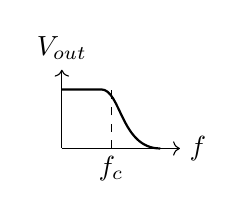
\begin{tikzpicture}[scale=0.5]
    \draw[->] (0,0) -- (3,0) node[right] {$f$};
    \draw[->] (0,0) -- (0,2) node[above] {$V_{out}$};
    \draw[thick] (0,1.5) -- (1,1.5) .. controls (1.5,1.5) and (1.5,0) .. (2.5,0);
    \draw[dashed] (1.25,0) -- (1.25,1.5);
    \node at (1.25,-0.5) {$f_c$};
\end{tikzpicture}
& Passes frequencies below cutoff $f_c$, blocks higher \\ \hline
\textbf{High Pass} & 
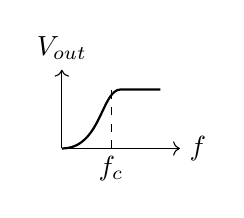
\begin{tikzpicture}[scale=0.5]
    \draw[->] (0,0) -- (3,0) node[right] {$f$};
    \draw[->] (0,0) -- (0,2) node[above] {$V_{out}$};
    \draw[thick] (0,0) .. controls (1,0) and (1,1.5) .. (1.5,1.5) -- (2.5,1.5);
    \draw[dashed] (1.25,0) -- (1.25,1.5);
    \node at (1.25,-0.5) {$f_c$};
\end{tikzpicture}
& Blocks frequencies below cutoff $f_c$, passes higher \\ \hline
\textbf{Band Pass} & 
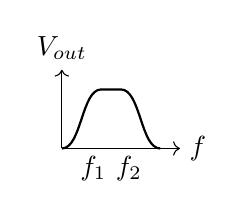
\begin{tikzpicture}[scale=0.5]
    \draw[->] (0,0) -- (3,0) node[right] {$f$};
    \draw[->] (0,0) -- (0,2) node[above] {$V_{out}$};
    \draw[thick] (0,0) .. controls (0.5,0) and (0.5,1.5) .. (1,1.5) -- (1.5,1.5) .. controls (2,1.5) and (2,0) .. (2.5,0);
    \node at (0.8,-0.5) {$f_1$}; \node at (1.7,-0.5) {$f_2$};
\end{tikzpicture}
& Passes frequencies between $f_1$ and $f_2$ \\ \hline
\textbf{Band Stop} & 
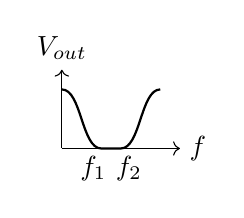
\begin{tikzpicture}[scale=0.5]
    \draw[->] (0,0) -- (3,0) node[right] {$f$};
    \draw[->] (0,0) -- (0,2) node[above] {$V_{out}$};
    \draw[thick] (0,1.5) .. controls (0.5,1.5) and (0.5,0) .. (1,0) -- (1.5,0) .. controls (2,0) and (2,1.5) .. (2.5,1.5);
    \node at (0.8,-0.5) {$f_1$}; \node at (1.7,-0.5) {$f_2$};
\end{tikzpicture}
& Blocks frequencies between $f_1$ and $f_2$ \\ \hline
\end{tabulary}
\end{center}

\begin{mnemonicbox}
\mnemonic{LHBS: Low lets low tones, High lets high tones, Band-pass selects middle, Band-Stop rejects middle}
\end{mnemonicbox}
\end{solutionbox}

\questionmarks{5(c) OR}{7}{Derive equation for designing a constant K low pass filters.}

\begin{solutionbox}
\textbf{Constant-K Low Pass Filter Design:}

\begin{center}
\begin{tabular}{cc}
\begin{circuitikz}[scale=0.8]
    \node at (2,2.5) {T-section};
    \draw (0,2) to[L, l=$L/2$] (2,2) to[L, l=$L/2$] (4,2);
    \draw (2,2) to[C, l=$C$] (2,0);
    \draw (0,0) -- (4,0);
\end{circuitikz} &
\begin{circuitikz}[scale=0.8]
    \node at (2,2.5) {$\pi$-section};
    \draw (0,2) to[L, l=$L$] (4,2);
    \draw (0,2) to[C, l=$C/2$] (0,0);
    \draw (4,2) to[C, l=$C/2$] (4,0);
    \draw (0,0) -- (4,0);
\end{circuitikz}
\end{tabular}
\captionof{figure}{Constant-K Low Pass Filter Sections}
\end{center}

\textbf{Design Theory:}
A constant-K filter has impedance product $Z_1Z_2 = R_0^2$ (constant) at all frequencies.

\textbf{Derivation Steps:}
\begin{enumerate}
    \item For a T-section low-pass filter:
       Series impedance $Z_1 = j\omega L$, Shunt impedance $Z_2 = 1/j\omega C$
    \item Product $Z_1Z_2 = L/C = R_0^2$ (constant $k^2$)
    \item Characteristic impedance at zero frequency: $R_0 = \sqrt{L/C}$
    \item Cut-off frequency occurs when $Z_1/4 + Z_2 = 0$ or $Z_1 = -4Z_2$ (Pass band condition in filter theory $-1 < Z_1/4Z_2 < 0$, cutoff at limit).
       More simply, cutoff $\omega_c$ is where $X_L = 2X_C$ for full section?
       Standard formula: $\omega_c = 2/\sqrt{LC}$
    \item From $R_0 = \sqrt{L/C}$ and $\omega_c = 2/\sqrt{LC}$:
       $L = R_0/\pi f_c$
       $C = 1/(\pi f_c R_0)$
\end{enumerate}

\textbf{Final Design Equations:}
\begin{itemize}
    \item Inductance: $L = R_0/(\pi f_c)$
    \item Capacitance: $C = 1/(\pi f_c R_0)$
    \item Cutoff Frequency: $f_c = 1/(\pi \sqrt{LC})$
\end{itemize}

\begin{mnemonicbox}
\mnemonic{One over Pi-Root-LC: The frequency where we Cut}
\end{mnemonicbox}
\end{solutionbox}

\end{document}

